\documentclass[10pt,halfparskip,DIV15]{scrartcl}

\usepackage{proposal}

\begin{document}

\pagestyle{empty}

\section*{Bachelor Assignment}

\begin{description}
	\item[Topic] Structural Analyser for Python
	\item[Date] 18 February 2008 – 6 June 2008
	\item[Students] ~ \\
		Reto Schüttel, \\
		Robin Stocker
	\item[Supervisor] ~ \\ 
		Peter Sommerlad \\
		Institute for Software IFS \\
 		University of Applied Sciences HSR Rapperswil

\end{description}

\vspace{-0.5cm}

\subsection*{Project Description}

Planning and analysing a program's structure and internal dependencies is a common task when working on larger projects. Such analysis helps to meet the defined architectural design goals or to find structural flaws like cyclic dependencies. A clear architecture becomes more and more important as software grows.

This project's goal is to develop a structural analyser for programs written in the Python programming language. The analyser should be able to parse an application's source code, analyse it and then generate a graph representing the internal structure of the project. Details which are usually not known until runtime have to be inferred during the analysis.

The following information will be provided by the analyser: 
\begin{itemize}
	\item All involved \emph{components}, like modules, packages, classes or methods
	\item \emph{Dependencies} between such components, caused by:
	\begin{itemize}
		\item method calls
		\item using variables/parameters/fields of a certain type
		\item inheritance
	\end{itemize}
	\item Module layout/structure
\end{itemize}

The generated data can be used by other programs for various further analysis. One example is Structure 101g developed by Headway Software which takes arbitrary dependency data and visualises it. 

\vspace{-0.1cm}

\begin{figure}[h] \centering
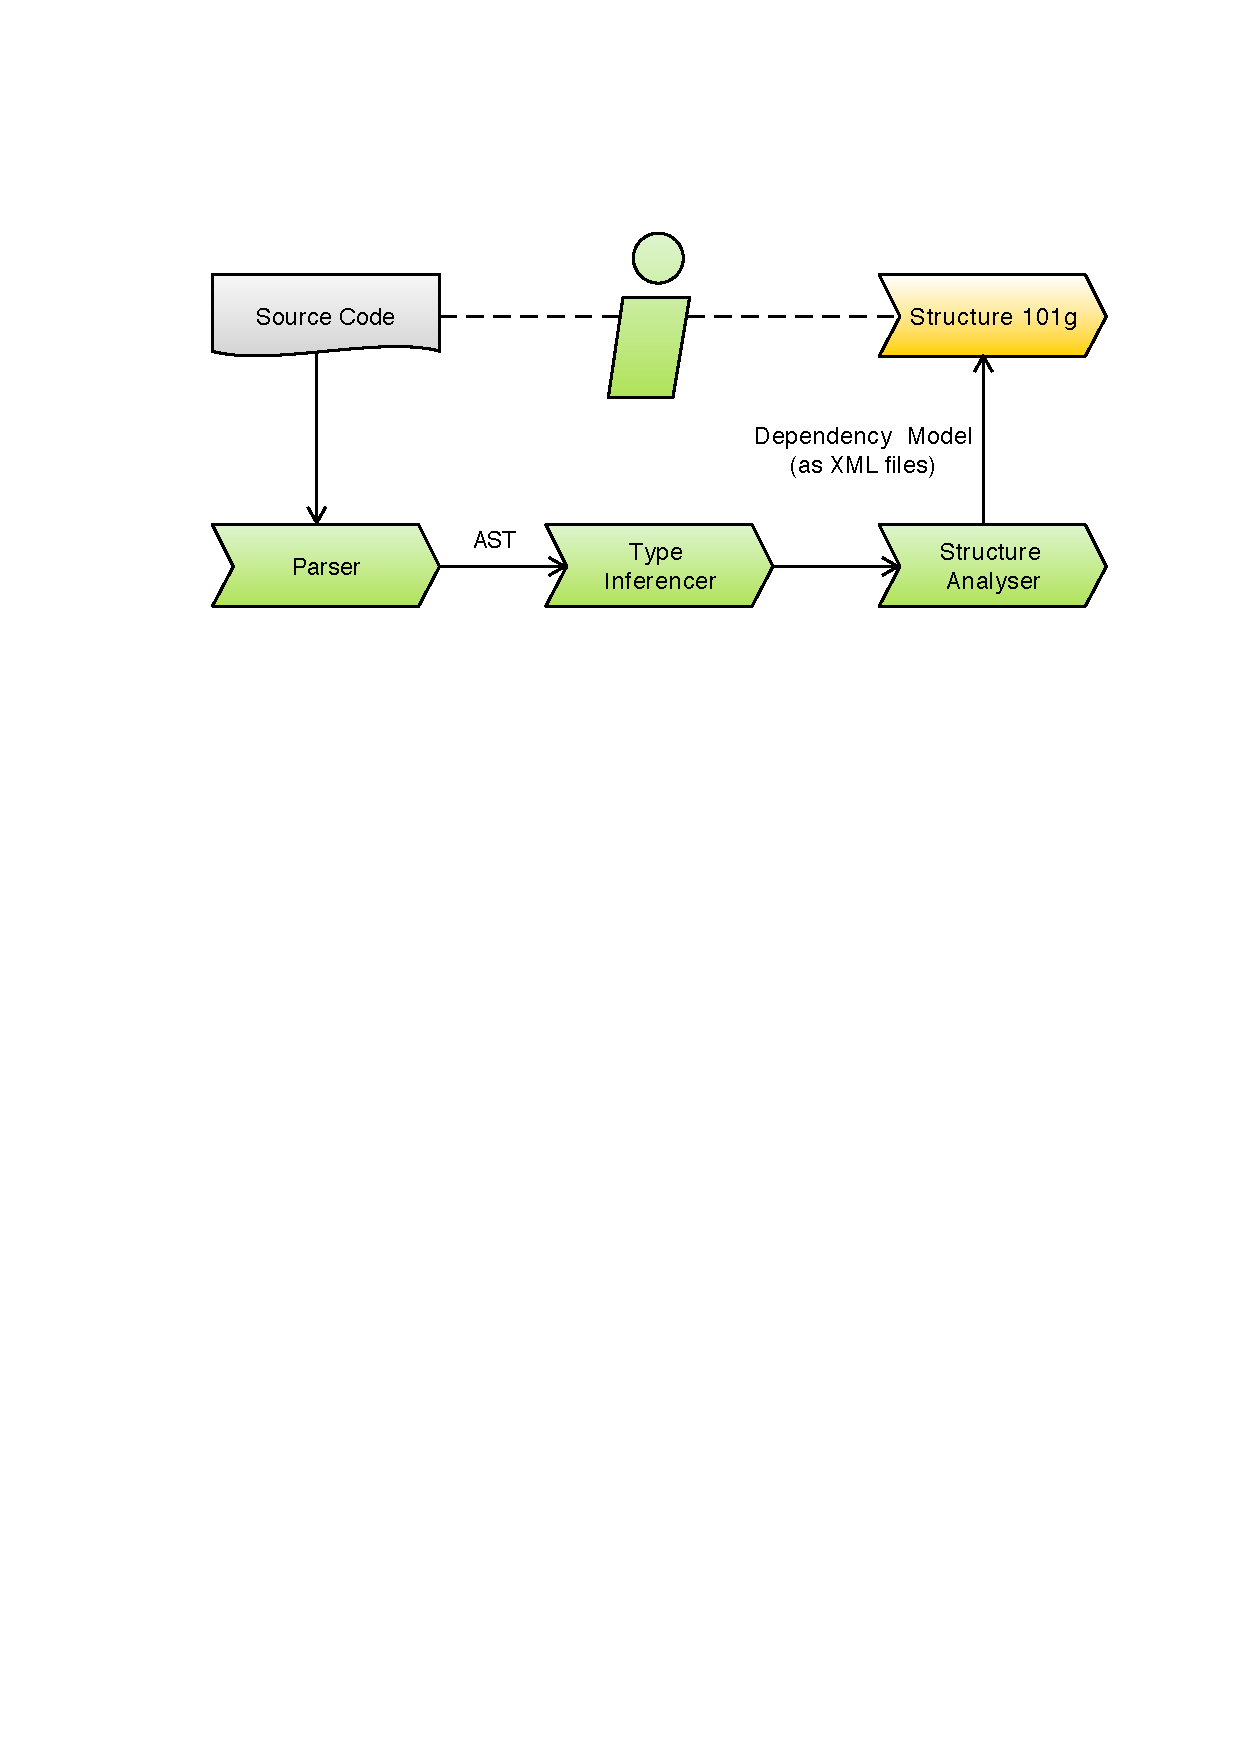
\includegraphics[width=0.6\textwidth]{big_picture}
\end{figure}

\vspace{-0.7cm}

\subsection*{Project Deliverables}

\begin{itemize}
	\item Bachelor Thesis Report
	\item Application
\end{itemize}






\end{document}
